One of the major successes of the electro-optical testing campaign on the summit (Run 7) was the mitigation of the persistence effect by changing the CCD operation voltage \citep{SITCOMTN-148}. This change greatly decreased the persistence signal to sub-ADU level. This was confirmed by taking uniform flat illumination images. Here we demonstrate the level of persistence by reducing the on-sky data where much sharper stars play a role.

On the night of May 15, 2025, LSSTCam observed a bright star on R22/S11, which is an e2v sensor, during BLOCK-T417 (CLT-001 Incremental Closed Loop w/ coma bending modes). The first panel of Figure \ref{fig:persistence} shows the bright star image (Image sequence 470) after applying the standard isrTask (correcting bias, dark, flat, linearity, defects, etc.) and calibrateImageTask (calibrating WCS, photometry, and removing sky background). The bright star saturated its footprint to the full well and bled charges across entire columns. This star could leave the persistence signal in the subsequent image (471), but there was no obvious persistence remaining (the second panel of Figure \ref{fig:persistence}; the same image process has been applied).

A stronger test is to apply the difference imaging technique. We used image 479 as a template for the difference imaging because the LSSTCam observed mostly the same field and there was no major bright star observed in the preceding images. We further applied `lsst.afw.math.warpExposure` with `lanczos3` to match the template image to the science image, and `lsst.ip.diffim.subtractImages.AlardLuptonSubtractTask` to solve the PSF in order to match the PSF shapes of two images and convolve the PSF to the best S/N image (here it was the template) and subtract the warped regularized template from the science image.

The result is shown in the right-most panel of Figure \ref{fig:persistence}. No persistence residue is obvious in the region where the bright star was located. There are residual bright stars and dark spots. The bright stars are the stars that are above the saturation, and the dark spots are associated with the saturation bleed in the template image.

The image was obtained in the z-band. The mean sky level for 471 reported by RubinTV was 21296.30 ADU. A study in the u-band, where the sky level is much lower, will be needed.

\begin{figure}[ht]
    \centering
    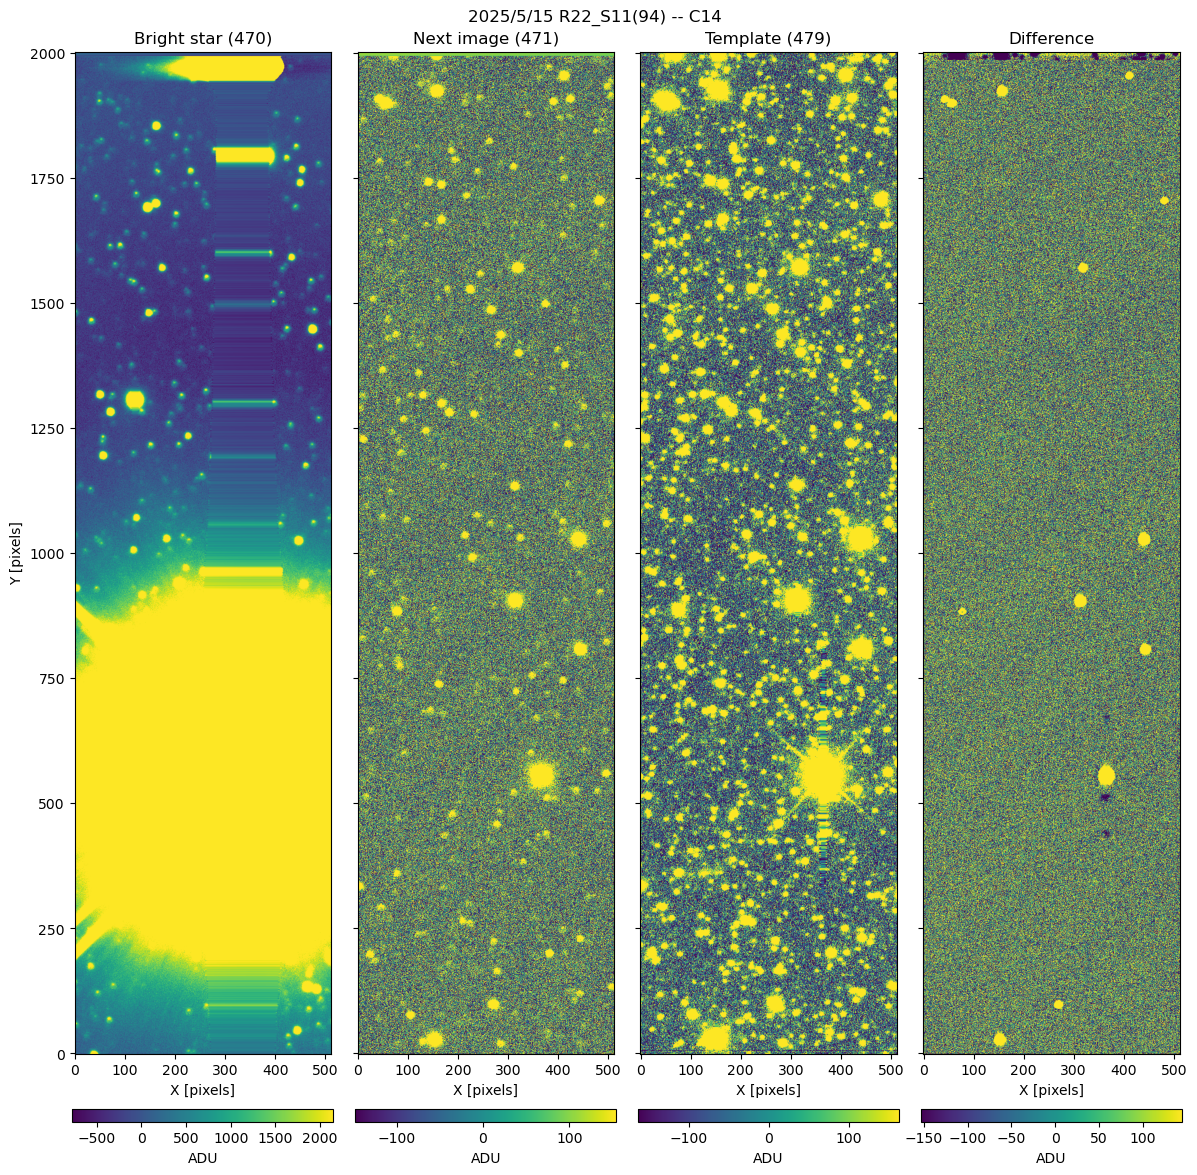
\includegraphics[width=1\linewidth]{onskyperformance//persistence/persistence.png}
    \caption{Demonstration of the absence of the persistence effect on an e2v sensor (R22/S11). The strip for channel 14 is cut out from an assembled CCD image. "Bright star" shows how the star appeared in the observation, "Next image" shows the next image after the bright star image, "Template" is a template image, and the Difference image is also shown.}
    \label{fig:persistence}
\end{figure}